\section{Introduction to quantum optics}\index{Quantum optics}\label{sec:intro_to_QO}

\famousquote{All the fifty years of conscious brooding have brought me no closer to answer the question, `What are light quanta?'. Of course today every rascal thinks he knows the answer, but he is deluding himself.}{Albert Einstein}
\newline

\dropcap{M}{uch} as the classical internet is heavily dependent upon optics to mediate communication, any future quantum internet will almost inevitably rely heavily on quantum optics to mediate quantum communication. It is therefore worth introducing the language and basic set of tools employed by quantum opticians.

%
% Discrete-variables
%

\subsection{Discrete-variables}\index{Discrete-variables}

Like most things in the quantum world, light is discretised into fundamental, indivisible particles called \textit{photons}\index{Photons} -- light quanta\index{Quanta}. This yields the most common representation for quantum states of light, referred to as the \textit{discrete-variables} (DV) picture\index{Discrete-variables}.

% Photon-number states

\subsubsection{Photon-number states}

The most basic optical quantum state comprising photons is the \textit{photon-number state}\index{Photon-number!States} or \textit{Fock state}. These states form a discrete basis, labelled by the integer number of photons in the state,
\begin{align}
\ket{n},\,n\in\mathbb{Z}^+.	
\end{align}
The special case of $\ket{0}$ is referred to as the \textit{vacuum state}\index{Vacuum state}, since it contains no photons.

The Fock states can be thought of as the energy levels in a quantum harmonic oscillator\index{Harmonic oscillators}, and the energy\index{Photons!Energy} of the $n$-photon Fock state is therefore given by,
\begin{align}
E_n = \left(n+\frac{1}{2}\right)\hbar\omega,
\end{align}
where $\omega$ is the optical frequency\index{Optical!Frequency} (in radians per second).

Any optical state in a single mode can be represented in the photon-number basis, which generalises to the multi-mode case in the obvious way, using a basis of composite photon-number states,
\begin{align}
	\ket{\vec{n}} = \ket{n_1}\otimes\ket{n_2}\otimes\cdots\otimes\ket{n_m},
\end{align}
for $m$ optical modes.

% Measurement

\subsubsection{Measurement}

A measurement in the photon-number basis is represented using photon-number projectors\index{Photon-number!Projectors},
\begin{align}
\hat\Pi_n = \ket{n}\bra{n},
\end{align}
which obey the usual completeness relation for measurement operators,
\begin{align}
\sum_{n=0}^\infty \hat\Pi_n &= \hat\openone.	
\end{align}

% Creation & annihilation operators

\subsubsection{Creation \& annihilation operators}\label{sec:creation_ann_ops}

In many cases it's convenient to represent states using photonic \textit{creation} ($\hat{a}^\dag$) and \textit{annihilation} ($\hat{a}$) operators\index{Creation operators}\index{Annihilation operators}. These (non-commuting) operators have the effect of acting upon a photon-number state and incrementing or decrementing its photon-number. Note that these operators are not unitary, and therefore do not represent legitimate quantum evolutions on their own. However, they may be employed to construct unitary operators representing physically legitimate evolution processes.

These operators satisfy the following basic algebraic properties:
\begin{align}
\hat{a}^\dag\ket{n} &= \sqrt{n+1}\ket{n+1},\nonumber\\
\hat{a}\ket{n} &= \sqrt{n}\ket{n-1},\nonumber\\
\hat{a}\ket{0} &= 0.
\end{align}
From this, it follows that an arbitrary Fock state can be expressed in terms of creation operators as,
\begin{align}
\ket{n} = \frac{1}{\sqrt{n!}}(\hat{a}^\dag)^n\ket{0}.
\end{align}
The creation and annihilation operators obey the commutation relation\index{Commutation relations},
\begin{align}
	[\hat{a},\hat{a}^\dag] &= 1,
\end{align}
where,
\begin{align}
[\hat{A},\hat{B}]=\hat{A}\hat{B}-\hat{B}\hat{A},
\end{align}
is the \textit{commutator}\index{Commutators} of two operators (operators that commute obviously necessarily exhibit \mbox{$[\hat{A},\hat{B}]=0$}). For multiple modes ($i$ and $j$) the different creation operators commute, as do the respective annihilation operators,
\begin{align}
[\hat{a}^\dag_i,\hat{a}^\dag_j] &= 0,\nonumber\\
[\hat{a}_i,\hat{a}_j] &= 0.
\end{align}
The physical interpretation of this property is that because photons are bosons, they are exchange-symmetric, and thus the physical state is invariant under swapping them.

% Photon-number operators

\subsubsection{Photon-number operators}\index{Photon-number!Operators}

A particularly useful and ubiquitous operator is the photon-number operator, defined as,
\begin{align}
\hat{n}=\hat{a}^\dag\hat{a},
\end{align}
which satisfies the eigenvalue relation\index{Eigenvalue equations} with photon-number states,
\begin{align}
\hat{n}\ket{n} = n\ket{n}.	
\end{align}
Treating it as a measurement observable\index{Observables}, the expectation value\index{Expectation values} of the photon-number operator, $\braket{\hat{n}}$, gives us the average measured photon-number when a state is measured in the photon-number basis, yielding the statistical average of the photon-number measurement outcome.

%
% Continuous-variables
%

\subsection{Continuous-variables}\index{Continuous-variables}

A completely alternate, but entirely equivalent formalism for the representation of quantum optical states is in the \textit{continuous-variables} (CV) picture. Here we no longer think in terms of a discretised photon-number basis, but in terms of a continuous basis in the complex plane, referred to as \textit{phase-space}\index{Phase-space}, completely analogous to the familiar classical phase-space. This alternate representation is introduced purely as a matter of convenience, since some states (typically referred to as CV states), are particularly well-suited to elegant representation in this picture, as are some types of evolution.

% Position & momentum operators

\subsubsection{Position \& momentum operators}

In the CV picture, instead of representing states using photonic creation operators, we express them in terms of the \textit{position} ($\hat x$)\index{Position operator} and \textit{momentum} ($\hat p$)\index{Momentum!Operator} operators, which are related to the creation and annihilation operators via,
\begin{align}
\hat x &=    \sqrt{\frac{\hbar}{2 \omega}}(\hat a + \hat a^\dag), \nonumber \\
\hat p &= -i \sqrt{\frac{\hbar  \omega}{2}}(\hat a - \hat a^\dag), 
\end{align}
where $\omega$ is the optical frequency\index{Optical!Frequency}. These operators obey the commutation relation\index{Commutation relations},
\begin{align}
[\hat x, \hat p] = i \hbar,
\end{align}
and satisfy the eigenvalue relations with the position and momentum eigenstates,
\begin{align}
\hat{x}\ket{x} &= x\ket{x},\nonumber\\
\hat{p}\ket{p} &= p\ket{p}.	
\end{align}
These eigenstates satisfy the completeness relations,
\begin{align}
\int_{-\infty}^\infty \ket{x}\bra{x}\,dx &= \hat\openone,\nonumber\\
\int_{-\infty}^\infty \ket{p}\bra{p}\,dp &	= \hat\openone.
\end{align}

The position and momentum operators represent the \textit{quadratures}\index{Quadratures} of a mode, and correspond to the real and imaginary components of a harmonic oscillator's\index{Harmonic oscillators} amplitude.

% Position & momentum representations

\subsubsection{Position \& momentum representations}\index{Position representation}\index{Momentum!Representation}

The \textit{position representation} of an optical state corresponds to expressing a state vector $\ket{\psi}$ in the position basis\index{Position representation},
\begin{align}
\ket{\psi} = \int \psi(x)\ket{x}\, dx.
\end{align}

Here the wave-function\index{Wave-functions} in the position representation\index{Position representation} is defined as,
\begin{align}
\psi(x) = \braket{x|\psi}.
\end{align}
The state can similarly be expressed via a \textit{momentum representation}\index{Momentum!Representation},
\begin{align}
	\ket\psi = \int {\tilde\psi}(p) \ket{p}\, dp,
\end{align}s
with wave-function\index{Wave-functions},
\begin{align}
	{\tilde\psi}(p) = \braket{p|\psi},\nonumber\\
\end{align}

The quadrature eigenstates\index{Quadratures!Eigenstates} are mutually related to one another by a Fourier transform\index{Fourier transform},
\begin{align}
\ket{x} &= \frac{1}{\sqrt{\pi}} \int_{-\infty} ^\infty e^{-2 i x p} \ket{p} \,dp,\nonumber \\
\ket{p} &= \frac{1}{\sqrt{\pi}} \int_{-\infty} ^\infty e^{2 i x p} \ket{x} \,dx.
\end{align}

% Coherent states

\subsubsection{Coherent states}\index{Coherent states}

A particularly ubiquitous state that emerges in CV representations is the \textit{coherent state}\index{Coherent states}, which closely approximates classical laser light\index{Lasers},
\begin{align}\index{Coherent states}
\ket{\alpha} = e^{-\frac{|\alpha|^2}{2}} \sum_{n=0}^\infty \frac{\alpha^n}{\sqrt{n!}} \ket{n},
\end{align}
where \mbox{$\alpha\in\mathbb{C}$} is the complex coherent amplitude. Alternately, coherent states can be defined as the eigenstates of the annihilation operator,
\begin{align}
\hat{a}\ket{\alpha} = \alpha\ket{\alpha}.
\end{align}
Writing the coherent amplitude as,
\begin{align}
	\alpha=re^{i\theta},
\end{align}
$r$ can be interpreted as the strength of the classical field, and $\theta$ as its local phase.

Note that the coherent state has indeterminate photon-number (and hence energy) -- it is in fact a coherent superposition of \textit{all} photon-numbers (except when \mbox{$\alpha=0$}). However, the \textit{mean} photon-number\index{Coherent states!Mean photon-number} is a useful quantity, given by,
\begin{align}
\bar{n} = \braket{\hat{n}} = |\alpha|^2.
\end{align}

% Phase-space representations

\subsubsection{Phase-space representations}\index{Phase-space}

We can graphically represent phase-space on the complex plane, where the two axes denote expectation values of the $\hat{x}$ and $\hat{p}$ operators. Unlike classical phase-space, in quantum phase-space states are `blobs'\index{Blobs} rather than points. The variance of these blobs represents the measurement uncertainty in a given direction, which is strictly non-zero in the quantum world, owing to the Heisenberg uncertainty principle\index{Uncertainty principle}.

The phase-space representation for a coherent state is a circular blob with mean $\alpha$ in the complex plane\index{Complex plane}, shown in Fig.~\ref{fig:phase_space}. Its variance is indicative of the quantum uncertainty\index{Uncertainty} of the field in the two quadrature directions. A coherent state is a \textit{minimum uncertainty state}\index{Minimum uncertainty state}, where the product of the variances in the two orthogonal directions is minimised. For other states it will be greater in general, but strictly not less.

\begin{figure}[!htbp]
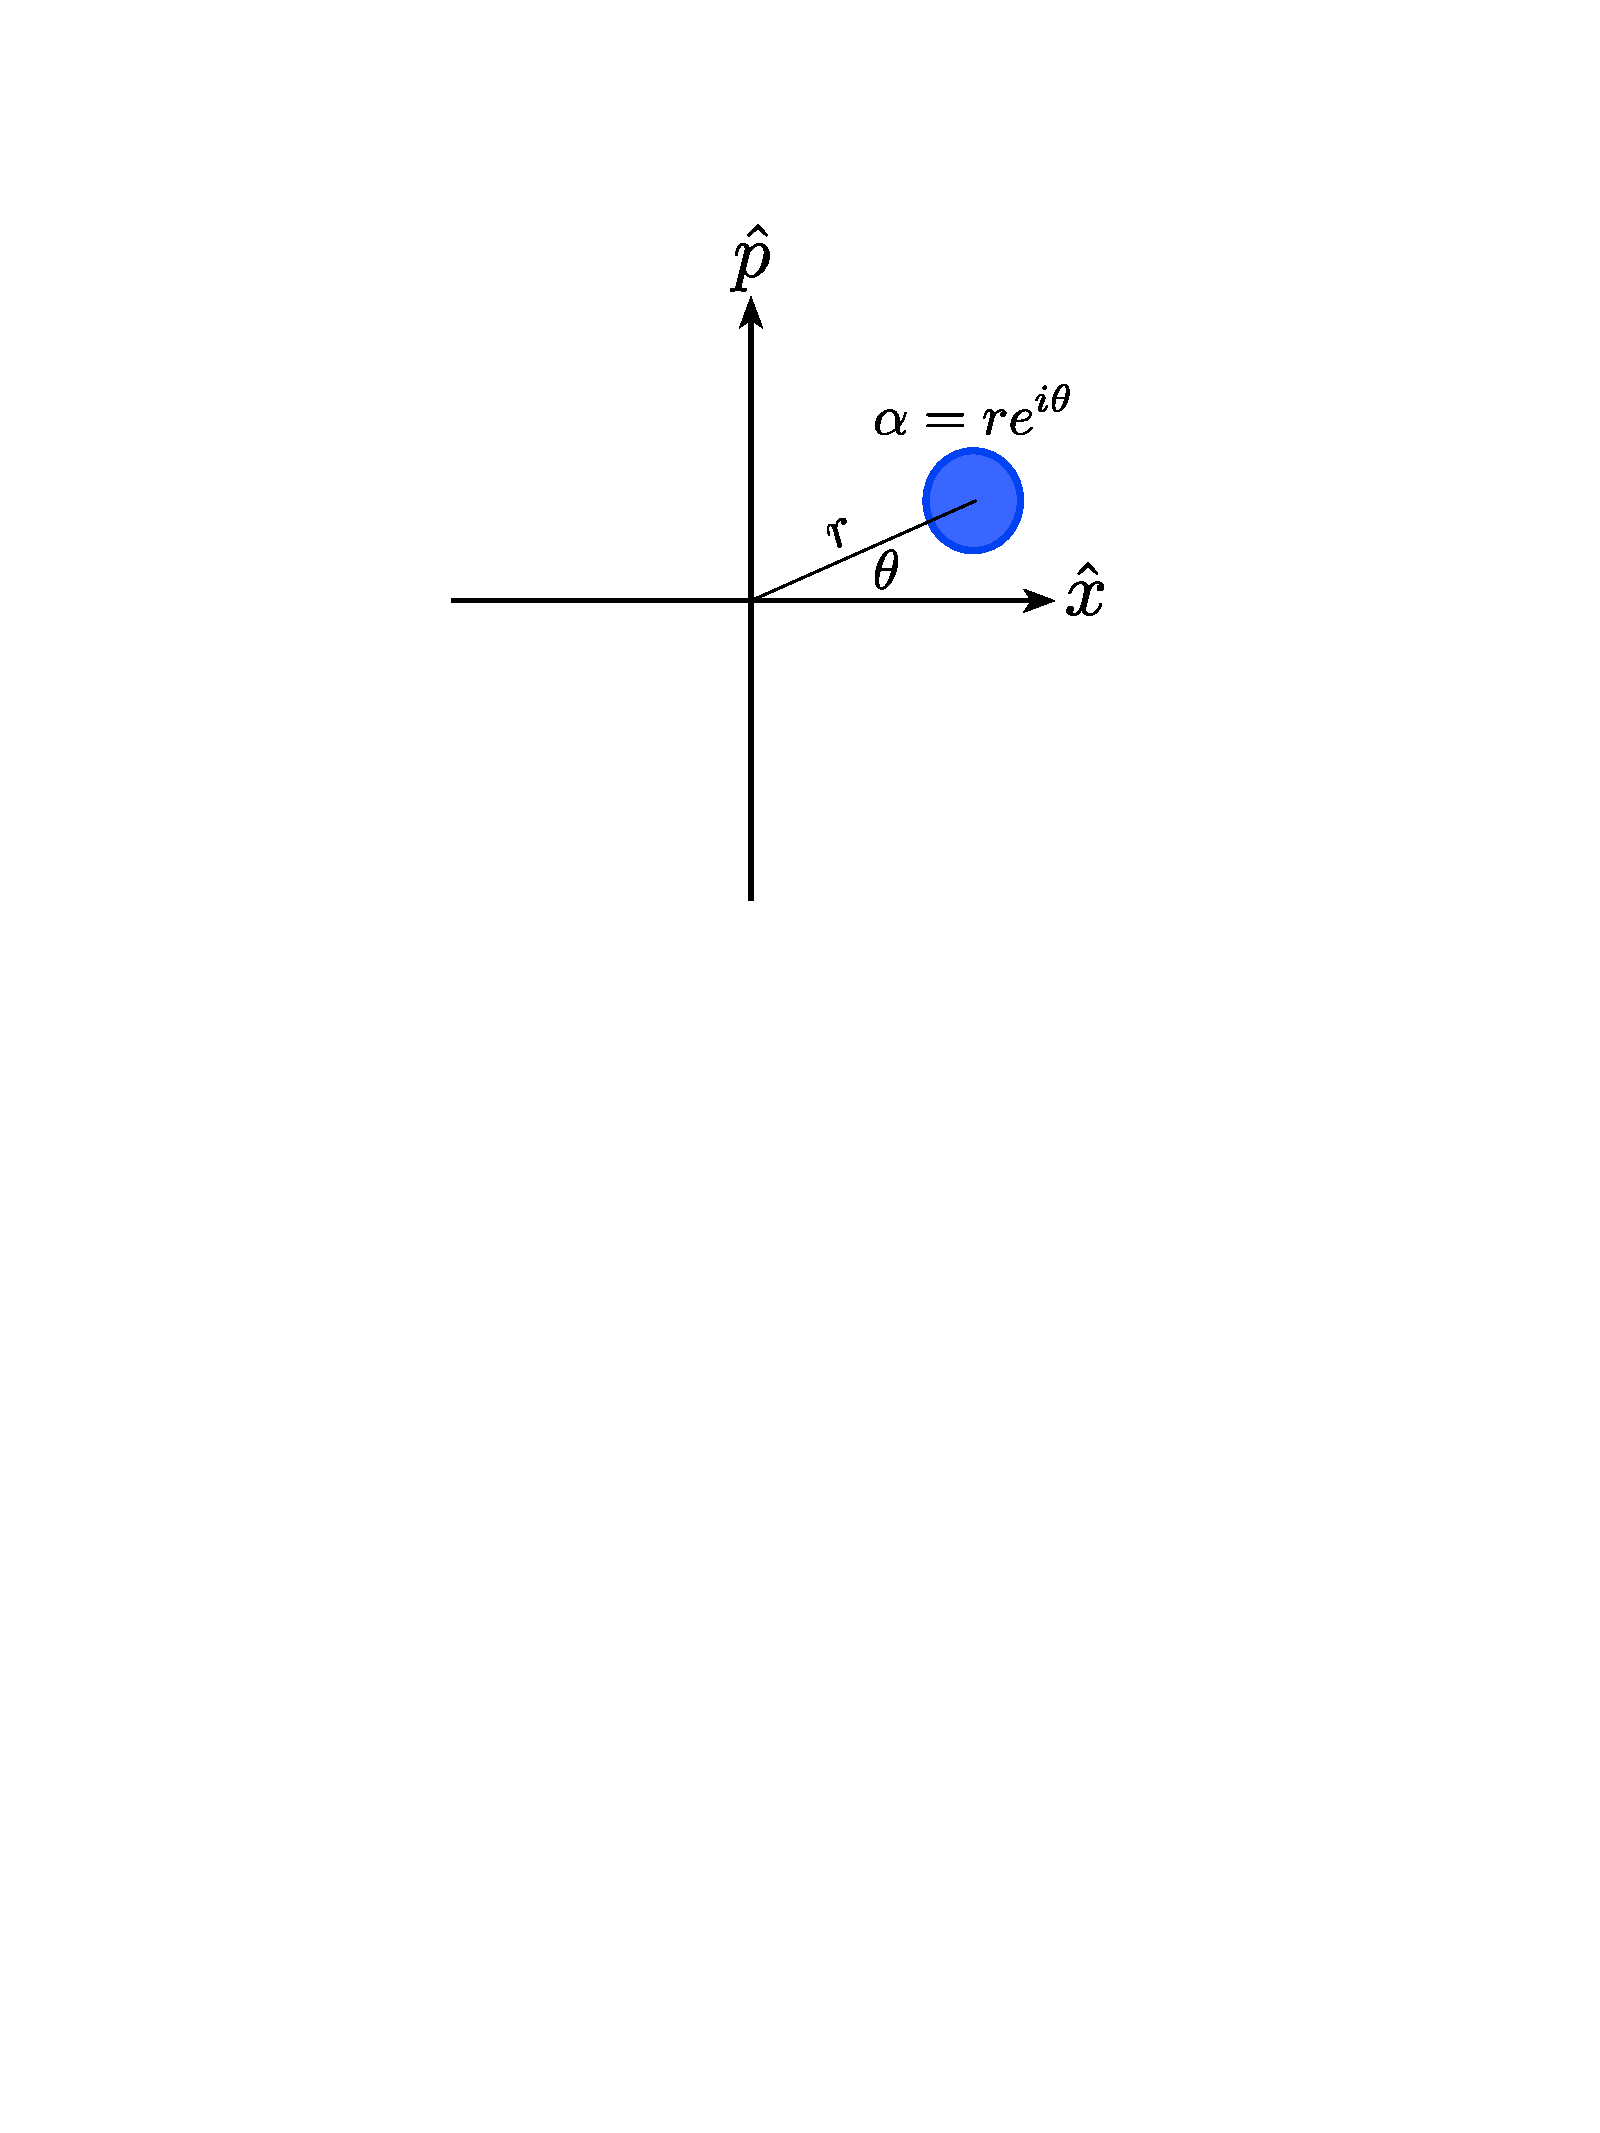
\includegraphics[clip=true, width=0.4\textwidth]{phase_space}
\captionspacefig \caption{Phase-space representation for a coherent state of complex amplitude \mbox{$\alpha=re^{i\theta}$}, where $r$ can be regarded as the field strength, and $\theta$ its phase.}\label{fig:phase_space}
\end{figure}

Beyond coherent states, represented by circular blobs, all manner of other geometries are available, allowing states such as \textit{squeezed states}\index{Squeezed states} (another useful type of CV state), which are rather complex to work with in the DV picture, to be elegantly graphically represented.

In phase-space, the evolution of a state under the accumulation of optical phase\index{Phase-space!Evolution} simply manifests itself as a rotation of the complex plane around the origin over time. Thus, the coherent state blob simply revolves around the origin. On the other hand, photon-number states manifest themselves as concentric rings in phase-space. Since this geometry is circular-symmetric, its phase-space representation is invariant under phase evolution.